\section{Distribution}
To distribute \doom, id software once again adopted the shareware model. A part of the game was given away for free (Episode I "Knee-Deep in the Dead ", made of nine maps) and players were encouraged to copy and give it away as much as possible. To this effect, they managed to cut and compress the game engine and the first episodes on only two 3$\nicefrac{1}{2}$-inch floppy disks.\\
\par 
A player happy with what she saw could send id Software a payment and receive the two remaining episodes ("The Shores of Hell" and its sequel, "Inferno") by the mail.\\
\par
\cfullimage{endoom.png}{"Title Screen" displayed at the end of each gaming session, left the player with instructions to follow in order to get more episodes.}
\par
Only this time they wanted to see things in a bigger way. Not only they wanted to be distributed via players, they also wanted to be in brick and mortar store. But they did not want to have to take care of boxes and inventory issues tied to physical distribution.\\
\par
 As it turned out there was a way to achieve this seemingly impossible task thanks to an idea from Jay Wilbur.\\
\par
\fq{We told the retailers "we don't care if you make money off this shareware demo". "Move it. Move it in mass quantities." The retailers couldn't believe their ears, no one had ever told them not to pay royalties.
But Jay was insistent. "Take DOOM for nothing, keep the profit". My goal is distribution. DOOM is going to
be Wolfenstein on steroids, and I want it far and wide.
I want you to stack DOOM high. In fact, I want you to
do advertising for it, too, because you're going to make money off it. So take this money that you might have given me in royalties and use it to advertise the fact that you're selling DOOM.}{Jay}\\
\par
John Romero shares the same memory and even elaborated on the creativity he witnessed.\\
\par
\fq{The challenge was: "How do we get Doom in the store? How do we get something free on shelves?\\
\par 
The idea was that the title screen of doom says "Suggested retail price \$9 dollars" on it and then we told the
companies that were already in the stores "if you put DOOM in the store in a box on the shelf you just keep all
the money. We don't want any of it just put it in a box and sell it".\\
\par 
Nutty, except that worked. It was everywhere. If you went into a CompUSA back then in 1994 you would see ten different boxes of doom and think they're all different games but they're all the same shareware game. Distributors ended up trying to make the best looking boxes to outperform their competitors because all they were allowed to sell was the shareware.}{John Romero}\\
\par

The success of the formula exceeded their wildest expectation. The shareware would find its way everywhere, even in the most suprising packages.\\
\par Despite manufacturing difficulties, book authors had the two floppies tapped at the end of book. The famous  "DooM Strategy guides" was among them. Magazines also jumped on the opportunity, they had to be wrapped in plastic bag to contain the two floppies.\\




%Ideally, to make distribution as easy as possible, the game would have fitted on one 3\nicefrac{1}{2}-inch floppy disk. Even though 650 KiB floppy reader were fading out in favor of 1,440 KiB floppies, because of the volume of assets, DooM shareware still used two disks.\\
\par
\cfullimage{floppies.png}{Two floppies containing Doom shareware. Notice how they were in fact bundled with the book "Survivor's Strategies and Secrets". The publisher paid no royalties to id Software to include their shareware.}
\par
The sofware packaging was a departure from the previous title. While Wolfenstein 3D shipped with a \cw{WOLF3D.EXE} engine an a multitude of \cw{.WL6} files, \doom had only two files. After installation, besides a few \cw{TXT} files, the game was made of the engine \cw{DOOM.EXE} and all assets in \cw{DOOM.WAD}.\\ 
\par
\def\angle{0}
\def\radius{3}
\def\cyclelist{{"orange","blue","red","green"}}
\newcount\cyclecount \cyclecount=-1
\newcount\ind \ind=-1


\begin{figure}[H]
\centering
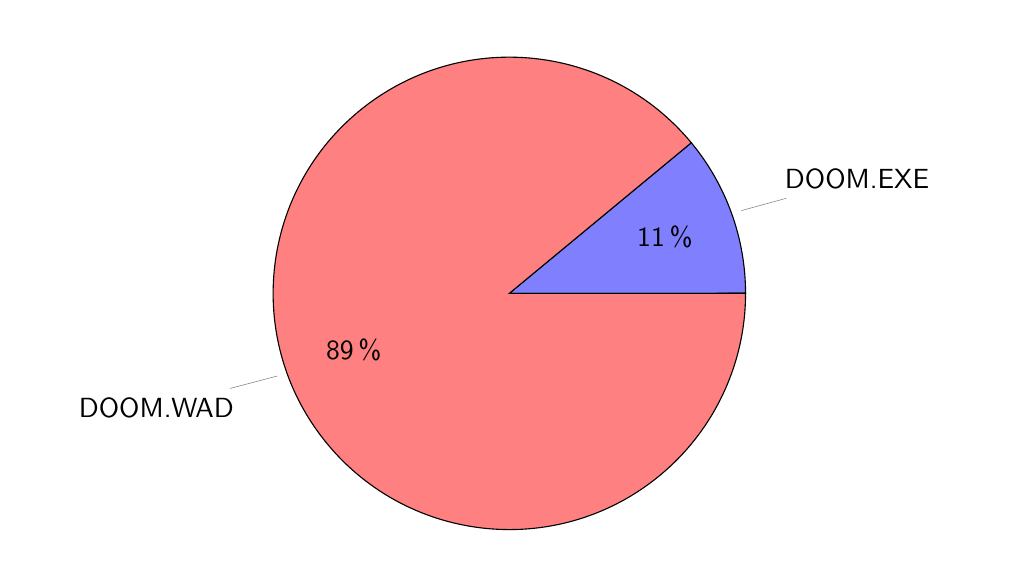
\begin{tikzpicture}[nodes = {font=\sffamily}]
  \node (a) at (6,0) {};
  \node (b) at (-6,0) {};
  \foreach \percent/\name in {
      11/DOOM.EXE,
      89/DOOM.WAD
    } {
      \ifx\percent\empty\else               % If \percent is empty, do nothing
        \global\advance\cyclecount by 1     % Advance cyclecount
        \global\advance\ind by 1            % Advance list index
        \ifnum3<\cyclecount                 % If cyclecount is larger than list
          \global\cyclecount=0              %   reset cyclecount and
          \global\ind=0                     %   reset list index
        \fi
        \pgfmathparse{\cyclelist[\the\ind]} % Get color from cycle list
        \edef\color{\pgfmathresult}         %   and store as \color
        % Draw angle and set labels
        \draw[fill={\color!50},draw={black}] (0,0) -- (\angle:\radius)
          arc (\angle:\angle+\percent*3.6:\radius) -- cycle;
        \node at (\angle+0.5*\percent*3.6:0.7*\radius) {\percent\,\%};
        \node[pin=\angle+0.5*\percent*3.6:\name]
          at (\angle+0.5*\percent*3.6:\radius) {};
        \pgfmathparse{\angle+\percent*3.6}  % Advance angle
        \xdef\angle{\pgfmathresult}         %   and store in \angle
      \fi
      
    };
\end{tikzpicture}
\end{figure}
\par
The registered version total size was 11,869,745 bytes, with 709,905 bytes dedicated to \cw{DOOM.EXE} and 11,159,840 bytes for \cw{DOOM.WAD}. Most of the volume was due to the rich graphical enviroment made of hundreds of sprites and textures.\\
\par


\par
\begin{figure}[H]
\centering
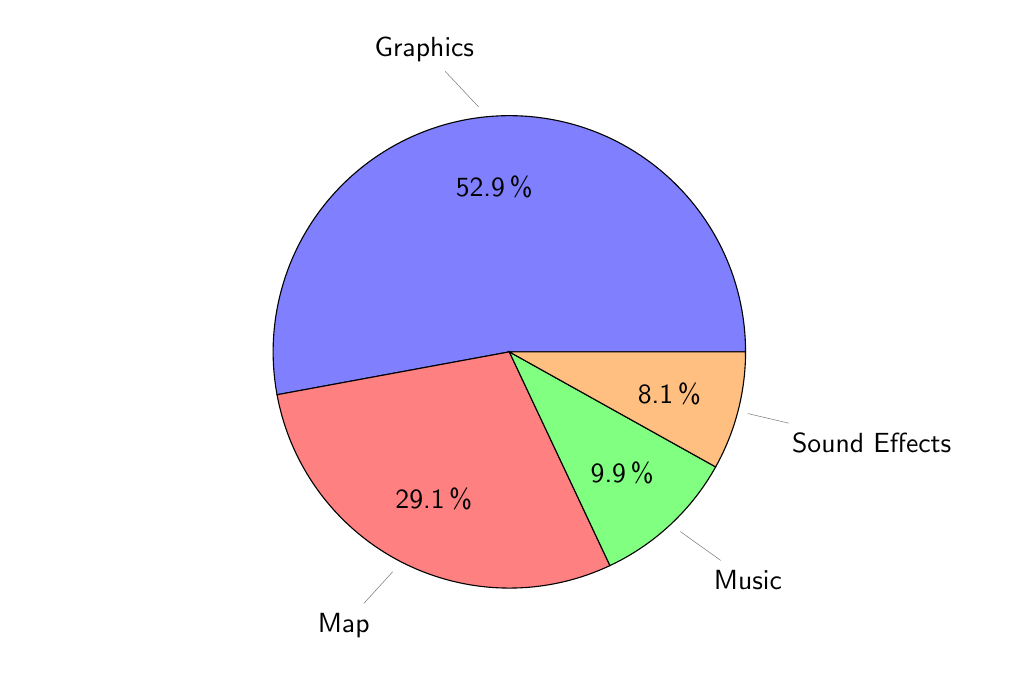
\begin{tikzpicture}[nodes = {font=\sffamily}]
\node (a) at (6,0) {};
  \node (b) at (-6,0) {};
  \foreach \percent/\name in {
      52.9/Graphics,
      29.1/Map,
       9.9/Music,
       8.1/{Sound Effects},
    } {
      \ifx\percent\empty\else               % If \percent is empty, do nothing
        \global\advance\cyclecount by 1     % Advance cyclecount
        \global\advance\ind by 1            % Advance list index
        \ifnum3<\cyclecount                 % If cyclecount is larger than list
          \global\cyclecount=0              %   reset cyclecount and
          \global\ind=0                     %   reset list index
        \fi
        \pgfmathparse{\cyclelist[\the\ind]} % Get color from cycle list
        \edef\color{\pgfmathresult}         %   and store as \color
        % Draw angle and set labels
        \draw[fill={\color!50},draw={black}] (0,0) -- (\angle:\radius)
          arc (\angle:\angle+\percent*3.6:\radius) -- cycle;
        \node at (\angle+0.5*\percent*3.6:0.7*\radius) {\percent\,\%};
        \node[pin=\angle+0.5*\percent*3.6:\name]
          at (\angle+0.5*\percent*3.6:\radius) {};
        \pgfmathparse{\angle+\percent*3.6}  % Advance angle
        \xdef\angle{\pgfmathresult}         %   and store in \angle
      \fi
    };
\end{tikzpicture}
\end{figure}



\subsection{WAD archive: Where Are the Data}
\label{wad_explained}
The goal of the \cw{WAD} format was partly to replace the OS filesystem but mostly to embrace the modding community. Each asset is stored in a structure called "lump" and packaged inside a file called a "wad". The file is made of three parts withc a header, a blob of data, and a directory at the end.\\

\par
\ccode{wad_structure.c}
\par
\trivia{The extension \cw{WAD} was coined by Tom Hall during an uncanny dialog. John Carmack was looking for a name for its archive format. Upong asking "How do you call a file Where's All the Data?", Tom responded immediately: "A WAD!" }\\
\par
\rawdrawing{wad_arch}
\par
The archive format was manipulated via two tools. \cw{lumpy} took a blob and packed it inside a lump, inside a \cw{WAD}. \cw{wadlink} took serveral \cw{WAD} and created/appended them into a single \cw{WAD}. The lump structure allowed to easily add or remove lumps. Appending a new one at the end was easy since only the small directory at the end had to be moved down.\\
\par
The most interesting aspect of the design was the ability for third party to inject their own lumps. \doom had a parameter allowing to load extra \cw{WAD} files which would be looked into before \cw{DOOM.WAD} when searching for a lump name. This mechanism allowed to customize everything (short for I.A which was baked in \cw{DOOM.EXE}). A custom \cw{WAD} containing a \cw{E1M1} lump could be used via as simple \cw{doom -file mylevel.wad} command.




